\documentclass[a4paper,10pt]{article}
\raggedbottom
\sloppy
\usepackage[utf8]{inputenc}
\usepackage{tabularx}
\usepackage[pdftex]{graphicx}
\graphicspath{{./Figures/}}
\usepackage[english]{babel}
\usepackage{romanbar}
\usepackage{varwidth}
\usepackage{framed}
\usepackage{cancel}
\usepackage{amsmath}
\usepackage{multirow}
\usepackage[usenames,dvipsnames]{xcolor}

\newcommand{\red}[1]{\textcolor{WildStrawberry}{#1}}
\definecolor{mymauve}{rgb}{0.58,0,0.82}
\definecolor{mygreen}{rgb}{0,0.6,0}
\definecolor{mygray}{rgb}{0.5,0.5,0.5}
\definecolor{bottomcol}{RGB}{222,222,222}

\usepackage{listings}
\lstset{
	language=SQL,
	basicstyle=\small\ttfamily,
	breaklines=true,
	frame=none,
	tabsize=2, 
	numbers=left,
	numbersep=8pt,
	xleftmargin=1.4em,
	commentstyle=\color{mygreen},
	numberstyle=\tiny\color{mygray},
	keywordstyle=\color{RoyalBlue},
	stringstyle=\color{mymauve},
	escapechar=\@, % for inserting LaTeX code in listing
	showstringspaces=false,	
	columns=fullflexible % reduce spacing between characters
}

\usepackage{float}

\usepackage{tikz}
\usetikzlibrary{shapes.misc} % for strike out function
\usetikzlibrary{shapes}
\usetikzlibrary{positioning}
\usetikzlibrary{calc}
\usepackage{tikz-qtree}
\tikzstyle{block} = [rectangle, draw, text centered, rounded corners]
\tikzstyle{class}=[
rectangle,
draw=black,
text centered,
anchor=north,
align=left,
text=black,
shading=axis,
bottom color=bottomcol,top color=white,shading angle=45]
\tikzstyle{line} = [draw,  ->]

\usepackage{stfloats}
\usepackage{enumitem}
\usepackage{tocloft}
\setlength{\cftfignumwidth}{2.65em}
\usepackage[margin=.75in]{geometry}

\usepackage{chngcntr}
\counterwithin{figure}{section}

\usepackage{enumitem}
\usepackage{color}
\usepackage{textcomp}
  
\setlength\parindent{0pt}
\setlist[enumerate]{itemsep=0mm}
\setlist[itemize]{itemsep=0mm}
\usepackage{mathtools}
\usepackage{amssymb}
\newlist{todolist}{itemize}{2}
\setlist[todolist]{label=$\square$}
\usepackage{pifont}
\newcommand{\cmark}{\ding{51}}%
\newcommand{\xmark}{\ding{55}}%
\newcommand{\done}{\rlap{$\square$}{\raisebox{2pt}{\large\hspace{1pt}\cmark}}%
	\hspace{-2.5pt}}
\newcommand{\wontfix}{\rlap{$\square$}{\large\hspace{1pt}\xmark}}
\usepackage{array}

\PassOptionsToPackage{hyphens}{url}\usepackage[
colorlinks=true,
urlcolor=PineGreen,
linkcolor=RoyalBlue,
citecolor=blue
]{hyperref}

% Include author name and title in pdf settings
\makeatletter
\AtBeginDocument{% \@author and \@title are only evaluated after the \begin{document}
	\hypersetup{
		pdftitle = {Introduction to Computer Graphics},
		pdfsubject = {Summary},
		pdfauthor = {Cyril Wendl}
	}
}
\makeatother

% header
\usepackage{fancyhdr}
\pagestyle{fancy}
\fancyhead[C]{}
\lhead[ \leftmark ]{Exam 2016 ICG}
%\chead{\nouppercase\leftmark}
\rhead[Wendl]{C. Wendl, \the\year}

\usepackage[super]{nth}

\sloppy
%title page
\author{Cyril Wendl}
\title{Exam 2016 ICG}
\begin{document}
\maketitle
\tableofcontents
\section{Parametric Curves}
\subsection{De Casteljau's algorithm}

\begin{figure}[H]
	\centering
	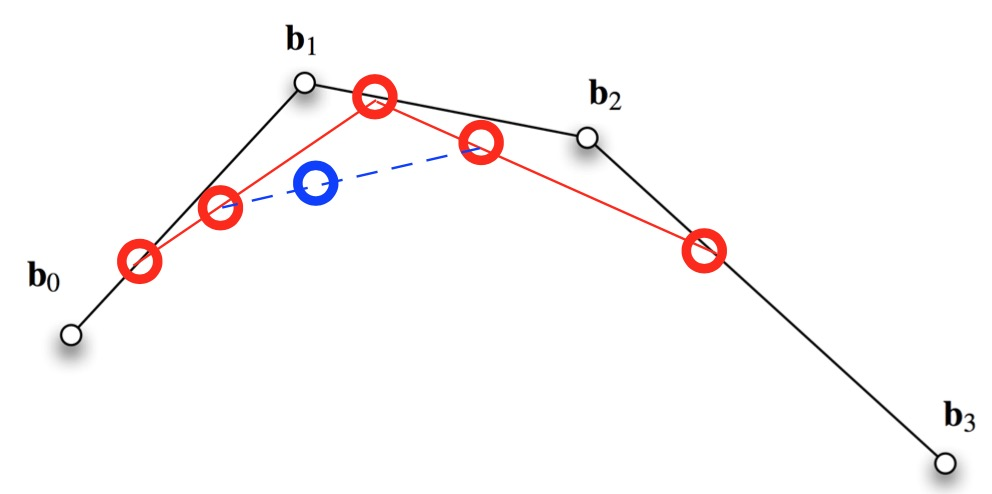
\includegraphics[width=.4\textwidth]{1-casteljau}
	\caption{De Casteljau's algorithm}
\end{figure}
blue: point at t=.25 and tangent\\
\subsection{Bézier curves - properties}
\textit{\textbf{(2 points)} Suppose the graph of a function $y = f (x)$ on interval [0, 1] can be represented by a Bézier curve $b(t)$. If there are 3 intersection points between $b(t)$ and the x-axis, what is the minimum degree of $b(t)$? Which property of Bézier curves can you use to explain your result?
}\\
\begin{figure}[H]
	\centering
	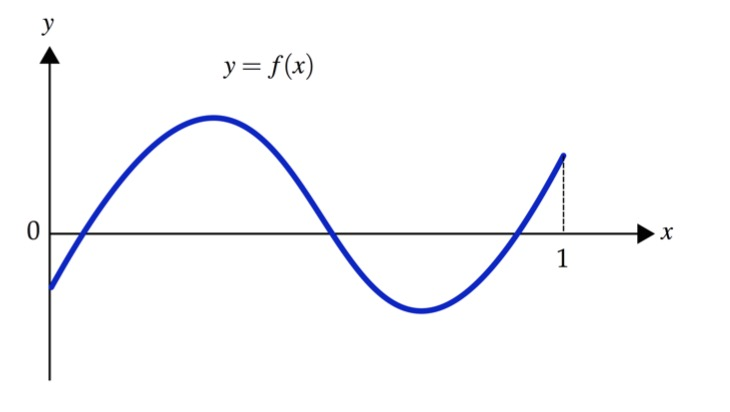
\includegraphics[width=.5\textwidth]{1-bezier}
\end{figure}

Bézier curve of degree n defined by n + 1 control points $P_0, P_1, P_2, ..., P_n$
\\$\rightarrow$ Minimum degree = 3, since we have 4 control points
\\$\rightarrow$ The variation diminishing property of Bézier curves is that they are smoother than the polygon formed by their control points

\textit{\textbf{(2 points)} From the graph above, can you determine the maximum degree of b(t)? Explain your answer.}\\

No, there could be infinitely many points along the line above and line would not change its shape if more points are added that lie exactly on the line. Therefore the maximum degree can be infinite.\\

\textit{\textbf{(3 points)} List three more properties of Bézier curves and provide a short explananation Bezier and Bernstein polynomials
tion of each one.}\\

\begin{enumerate}
	\item Affine invariance: it is similar to compute an affine transformation of all the points of the curve or only the control points.
	\item Invariance under affine transformation: for affine transformations such as scaling or rotation, Bezier curves keep their properties
	\item Convex hulls
	\item Endpoint interpolation: the first and the last points of a Bezier curve defined by points P0,P1,…PN are P0 and PN
	\item Symmetry: The same Bezier curve shape is obtained if the control points are specified in the opposite order.
	\item Linear precisions: if the control points are uniformly distributed on a straight line joining two points $p$ and $q$, the Bézier Curve is a straight line linearly parametrized.
\end{enumerate}
\begin{itemize}
	\item \url{https://people.eecs.ku.edu/~miller/Courses/IntroToCurvesAndSurfaces/BezierCurveProperties.html}
\end{itemize}

\subsection{Bezier and Bernstein polynomials}
\textit{Every polynomial curve $c(t)\in  \mathbb{R}^2$ of degree n with parameter $t \in [0, 1]$ can be expressed by a Bézier curve $b(t) = \sum_{i=0}^n B_i^n(t)b_i$ with corresponding Bézier control points $b_0,...,b_n$ and Bernstein polynomials}\\

\[B_i^n(t)=\binom{n}{i}t^i(1-t)^{n-i},\binom{n}{i}=\frac{n!}{i!(n-i!)}\]

\textit{\textbf{(1 point)} Write down the formula of a cubic Bézier curve with control points ($b_0,b_1,b_2,b_3$) using Bernstein polynomials.}\\


\[\begin{aligned} 
B_{0,3}&=\frac{3!}{0!(3-0)!}t^0(1-t)^{3}=(1-t)^{3}\\
B_{1,3}&=\frac{3!}{1!(3-1)!}t^1(1-t)^{2}=3t(1-t)^{2}\\
B_{2,3}&=\frac{3!}{2!(3-2)!}t^2(1-t)^{1}=3t^2(1-t)\\
B_{3,3}&=\frac{3!}{3!(3-3)!}t^3(1-t)^{0}=t^{3}\\
\Rightarrow b(t)&=(1-t)^3b_0+3t(1-t)^{2}b_1+3t^2(1-t)b_2+t^3b_3
\end{aligned}\]
\textit{\textbf{(5 points)} Prove that the derivative of a cubic Bézier curve with control points ($b_0,b_1,b_2,b_3$) is also a Bézier curve. What is the polynomial order of the derivative?}
\[\begin{aligned} 
\frac{d}{dt}b^n(t)&=\sum_{i=0}^nb_i\frac{d}{dt}B_i^n(t)\\
\frac{d}{dt}B_i^n(t)&=n(B_{i-1}^{n-1}(t) - B_{i}^{n-1}(t))\\
\frac{d}{dt}b^n(t)&=n\sum_{i=0}^{n-1} \underbrace{(b_{i+1}-b_i)}_{\Delta b_i}B_i^{n-1}(t)\\
\frac{d}{dt}b^3(t)&=3\sum_{i=0}^{2} (b_{i+1}-b_i)B_i^{2}(t)\\
&=3(\Delta b_0(1-t)^2+ 2\Delta b_1 t (1-t) +\Delta b_2t^2)\\
& \Rightarrow \text{second order}
\end{aligned}\]
\textit{\textbf{(3 points)} Prove the partition of unit property $\sum_{i=0}^nB_i^n(t)=1$ for $n=2$.}
\[\begin{aligned} 
\sum_{i=0}^2B_i^2(t)&=t^2+2t(1-t)+(1-t)^2\\
&=\cancel{t^2}+\cancel{2t}-\cancel{2t^2}+1-\cancel{2t}+\cancel{t^2}\\
&=1
\end{aligned}\]

\section{Projections and Transformations}
\subsection{Rotation matrices}
\textit{\textbf{(2 points)} 2D rotation matrices are defined as $R=\begin{bmatrix}
	\cos(\alpha)&-\sin(\alpha)\\ 
	\sin(\alpha)&\cos(\alpha)
	\end{bmatrix}$. Prove that any 2D rotation matrix is orthonormal.}\\

Definition of orthonormal:
\[R^T=R^{-1}\Rightarrow\det(R)=1\]
\[\det(R)=\underbrace{\cos(\alpha)^2+\sin(\alpha)^2}_{=1}\]
\textit{\textbf{(1 points)} Are there other orthonormal matrices that are not rotations of the form above? If yes, give an example.}\\

Reflection matrix
\[R=\begin{bmatrix}
\cos(\alpha)&\sin(\alpha)\\ 
\sin(\alpha)&-\cos(\alpha)
\end{bmatrix}\]

\textit{\textbf{(2 points)} Prove that the inverse of a rotation matrix is its transpose.}\\

\[\begin{aligned}
\because \det(R)&=1\\
R^{-1}&=\frac{1}{1}\begin{bmatrix}
\cos(\alpha)&\sin(\alpha)\\ 
-\sin(\alpha)&\cos(\alpha)
\end{bmatrix}\\
&=R^T
\end{aligned}\]


\textit{\textbf{(2 points)} Two 2D vectors v and n are orthogonal. Show that their orthogonality is preserved under a rotation R. (Hint: express their relationship in terms of a dot product).}\\

\[\begin{aligned} 
A&=\begin{bmatrix}
A_y\\ 
A_z
\end{bmatrix},B=\begin{bmatrix}
B_y\\ 
B_z
\end{bmatrix}\\
\overline{A}&=\begin{bmatrix}
\cos(\alpha) & -\sin(\alpha)\\ 
\sin(\alpha) &\cos(\alpha)
\end{bmatrix}
\begin{bmatrix}
A_y\\ 
A_z
\end{bmatrix}=
\begin{bmatrix}
\cos(\alpha)A_y-\sin(\alpha)A_z\\ 
\sin(\alpha)A_y+\cos(\alpha)A_z
\end{bmatrix},\\
\overline{B}&=
\begin{bmatrix}
\cos(\alpha)&-\sin(\alpha)\\ 
\sin(\alpha)&\cos(\alpha)
\end{bmatrix}
\begin{bmatrix}
B_y\\ 
B_z
\end{bmatrix}=\begin{bmatrix}
\cos(\alpha)B_y-\sin(\alpha)B_z\\ 
\sin(\alpha)B_y+\cos(\alpha)B_z
\end{bmatrix},\\
\overline{A}\cdot\overline{B}&=A_yB_y\cos(\alpha)^2-\cancel{A_yB_z(\cos(\alpha)\sin(\alpha))}-\cancel{A_zB_y(\sin(\alpha)\cos(\alpha))}+A_zB_z(\sin(\alpha)^2))\\
&+A_yB_y\sin(\alpha)^2+\cancel{A_yB_z(\cos(\alpha)\sin(\alpha))}+\cancel{A_zB_y(\sin(\alpha)\cos(\alpha))}+A_zB_z(\sin(\alpha)^2))\\
&=A_yB_y(\underbrace{\cos(\alpha)^2+sin(\alpha)^2}_{=1})+A_zB_z(\underbrace{\cos(\alpha)^2+sin(\alpha)^2}_{=1})\\
&=A_yB_y+A_zB_z
\end{aligned}\]
Or, a bit shorter:
\[n^Tv=0\Rightarrow(Rn)^T(Rv)=n^TR^TRv=n^Tv=0\]

\textit{\textbf{(2 points)} An object is rendered on the screen by multiplying its vertices by the model, view, and projection matrices: $\tilde{v} = PVMv.$ If you are given $\tilde{v}$, how do you compute its world coordinates?}\\

\[v_{world}=Mv=(PV)^{-1}\tilde{v}\]

\subsection{Perspective Projection}
\textit{\textbf{(2 points)} You are given a 2D set up as shown below. The camera is at the origin looking down $z$. The image plane is at $z = d$. Derive the screen space position $y_s$ of
the point ($y_w,z_w$).}\\

\begin{figure}[H]
	\centering
	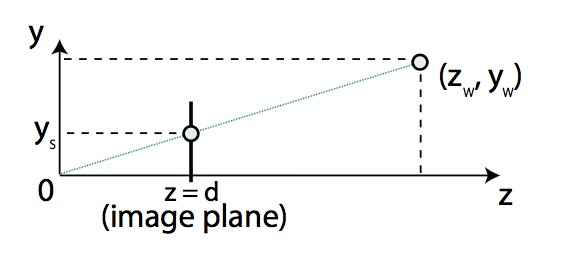
\includegraphics[width=.3\textwidth]{2-perspective}
\end{figure}
Because of the triangle similarity we have:
\[\begin{aligned}
&\frac{y_s}{d}=\frac{y_w}{z_w}\\
&\Rightarrow y_s=d\frac{y_w}{z_w}
\end{aligned}\]
\textit{\textbf{(2 points)} Generalize the previous question to the 3D setup. That is, derive the expression of the image plane coordinates ($x_s,y_s$) for the world coordinate point
($x_w,y_w,z_w$).}

\[x_s=d\frac{x_w}{z_w}, y_s=d\frac{y_w}{z_w}\]

\textit{\textbf{(2 points)} Is this transformation affine? (briefly justify your answer)}\\

No, you cannot  perform a division between elements of the same vector (e.g. $x_w/z_w$) with an affine transformation.\\

\textit{\textbf{(2 points)} Explain how homogeneous coordinates can be used to represent the perspective transformation above in matrix form?}\\

\[\begin{bmatrix}
d&&\\
&d&\\
&&1\\
\end{bmatrix}
\begin{bmatrix}
x_w\\
y_w\\
z_w\\
\end{bmatrix}=
\begin{bmatrix}
dx_w\\
dy_w\\
z_w\\
\end{bmatrix}\overset{hom.div.}{=}
\begin{bmatrix}
dx_w/z_w\\
dy_w/z_w\\
\end{bmatrix}\]

\subsection{Concatenating Affine Transformations}
\textit{\textbf{(3 points)}Derive the 3 $\times$ 3 homogeneous matrix that achieves the transformation in the figure.}\\

\begin{figure}[H]
	\centering
	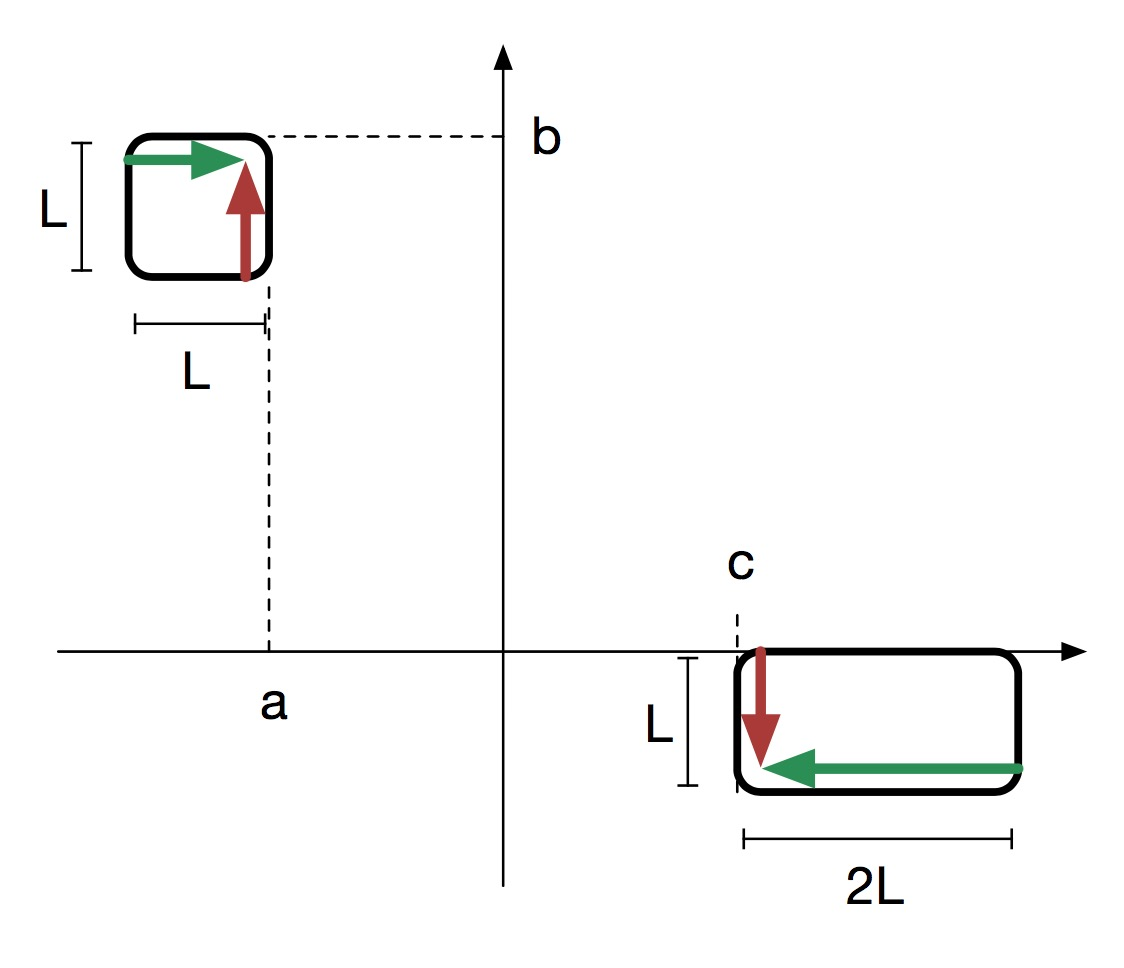
\includegraphics[width=.2\textwidth]{2-3-transformation}
\end{figure}
\begin{enumerate}
	\item $M_1$: translate (-a, -b)
	\item $M_2$: scale (-2, -1, 1)
	\item $M_3$: translate to (c, L).
\end{enumerate}
$M$=$M_3M_2M_1$
\[\begin{aligned}
M3&=\begin{bmatrix}
1 & 0 & c\\ 
0 & 1 & L\\ 
0 & 0 & 1
\end{bmatrix}
M_2=\begin{bmatrix}
-2 & 0 & 0\\ 
0 & -1 & 0\\ 
0 & 0 & 1
\end{bmatrix}
M_1	=\begin{bmatrix}
1 & 0 & -a\\ 
0 & 1 & -b\\ 
0 & 0 & 1
\end{bmatrix}\\
M&=M_3M_2M_1=(M_3M_2)M_1=\begin{bmatrix}
-2 & 0 & c\\ 
0 & -1 & L\\ 
0 & 0 & 1
\end{bmatrix}\cdot\begin{bmatrix}
1 & 0 & -a\\ 
0 & 1 & -b\\ 
0 & 0 & 1
\end{bmatrix}\\
&=\begin{bmatrix}
-2 & 0 & 2a +c\\ 
0 & -1 & -b+L\\ 
0 & 0 & 1
\end{bmatrix}
\end{aligned}\]
\textit{\textbf{(2 points)} Consider the following affine transformation (note that the \nth{3} dimension is not modified): $M = \begin{bmatrix}
	0&-1&0\\
	1&2&0\\
	0&0&1\\
\end{bmatrix}$. If a triangle is transformed with this matrix, how will its area change?}\\
	
Use only the upper-left 2x2 part of M. The triangle area will not change. The area is preserved if the transformation matrix has a determinant of 1.\\

%TODO prove

\textit{\textbf{(1 points)} How can you in general check if an affine transformation matrix pre- serves the area?
}\\

The area is preserved if the transformation matrix has a determinant of 1.

\subsection{Rasterizing Planar Reflections}
\textit{\textbf{(5 points)} The following list shows the possible steps (in order) necessary to render the reflection of the trees in the skycraper, as seen by the camera in the accompanying figure. Note that backface culling is enabled. Tick the boxes of the correct ones. 0.5 point for marking a correct statement, -0.5 point for marking an incorrect statement.}\\
\begin{figure}[H]
	\centering	
	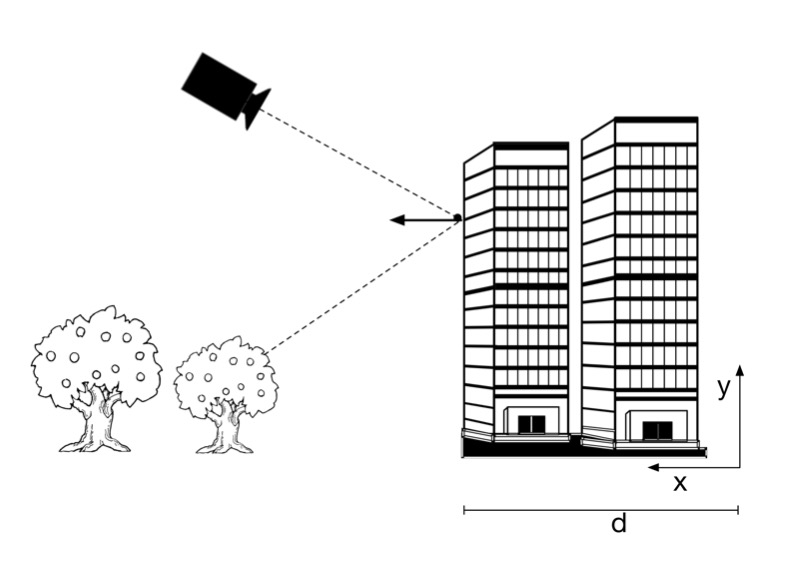
\includegraphics[width=.3\textwidth]{2-4-rasterizing}
\end{figure}
\begin{todolist}
	\item[\done] Prepare a framebuffer and bind it.
	\item Translate the view matrix by (d, 0, 0).
	\item Set the model matrix of the scene to: $\begin{bmatrix}
	-1 & 0 & 0 & 2d\\
	0 & 1 & 0 & 0\\
	0 & 0 & 1 & 0\\
	0 & 0 & 0 & 0
	\end{bmatrix}$
	\item[\done] Change the front face vertex order to clockwise.
	\item[\done] Set the model matrix of the scene to: $\begin{bmatrix}
	-1 & 0 & 0 & -2d\\
	0 & 1 & 0 & 0\\
	0 & 0 & 1 & 0\\
	0 & 0 & 0 & 0
	\end{bmatrix}$
	\item[\done] Translate the view matrix by (-d, 0, 0).
	\item Translate the view matrix by (0, d, 0).
	\item Set a clipping plane with equation (1, 0, 0, d).
	\item[\done] Set a clipping plane with equation (0, 1, 0, d).
	\item[\done] Render the scene.
	\item[\done] Unbind the framebuffer and set it as the texture of the skyscraper.
	\item[\done] Bind the main framebuffer (with id 0).
	\item[\done] Set the model matrix to Id.
	\item Set the model matrix to (-Id).
	\item[\done] Disable the specular materials in the scene.
	\item[\done] Reset the clipping planes, vertex order, lighting, view matrix to default. 
	\item[\done] Render the scene.
\end{todolist}

\section{Textures, Rasterization and Visibility}
\subsection{Rasterization}
\textit{In two sentences, quickly describe the painter's algorithm}\\

Sort polygons from back to front, and paint in that order. that leads to overwriting some of the already
filled parts.\\

\textit{ Complete the pseudo code to implement the z-buffer algorithm.}\\

\begin{lstlisting}[language=C]
// zbuffer[.,.]: R/Waccess
// framebuffer [ . , . ] : Read access
for (each polygon P) :
	for (each pixel (x,y,z) in P) :

	if (z < zbuffer(x,y)){
		framebuffer[x,y]=rgb; // write pixel's color to frame buffer
		zbuffer(x,y)=pixel(z);// update depth buffer
	}
\end{lstlisting}
04-Lighting slide 4\\

\textit{\textbf{(3 points)} The z-buffer algorithm has two main advantages over the painter’s algorithm? Describe and explain them.}
\begin{enumerate}
	\item It processes one object at a time, doesn’t require sorting of objects and avoids nested splitting
	\item It is very easy to implement and can be put in the hardware
\end{enumerate}

Sorting from back to front is not always possible without splitting polygons, and sorting is  $O(n \log n)$. Z-buffer is constant time and never ambiguous.\\

\url{http://www.cs.cmu.edu/afs/cs/project/anim/ph/463.96/pub/www/notes/zbuf.2.pdf}\\

\textit{\textbf{(2 points)} Barycentric coordinates can be used for simple 2D rasterization of a trisangle. Complete the following pseudo code for rasterizing one triangle.}\\
\begin{lstlisting}[language=C]
// You can use
// set pixel(x,y) to fill a pixel
// (a,b,c)=bary_coords(x,y) to compute barycentric coordinates within the triangle
 for (all x): 
 	for (all y):
 	(a,b,c)=bary_coords(x,y)
		if (a in [0,1] and b in [0,1] and c in [0,1])
			set_pixel (x,y)
\end{lstlisting}

\textit{\textbf{(3 points)} We have a triangle with vertices A,B,C. A point on the triangle’s plane can be represented with barycentric coordinates as $P = \alpha A + \beta B + \gamma C$. Sketch the three following regions:}
\begin{figure}[H]
	\centering
	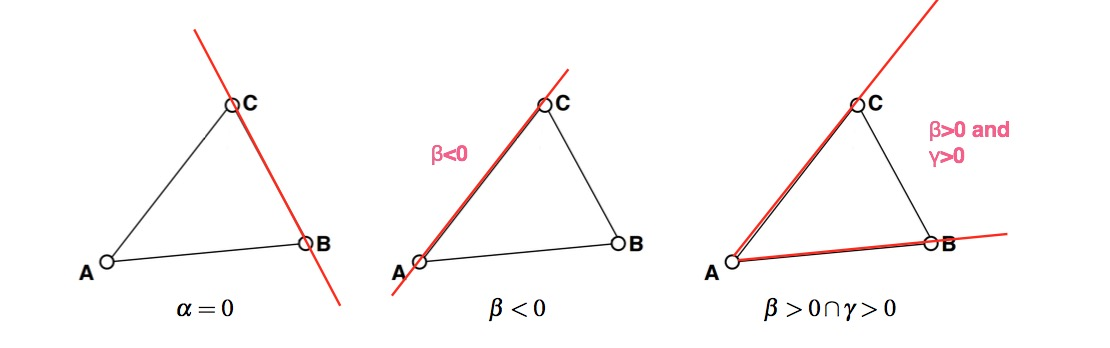
\includegraphics[width=.7\textwidth]{3-textures}
\end{figure}
\subsection{Texturing}
\textit{\textbf{(3 points)} Your program renders a quad whose texture coordinates ``\lstinline|in vec2 uv|'' are $\in [0, 1]$. Write a fragment shader (GLSL code) that generates a 8 $\times$ 8 checkerboard texture in blue and red.}\\
\begin{lstlisting}[language=C]
in vec2 uv;
out vec3 color;
		void main() {
		float grid_size = 8.0f;// remapping [0,1] to [0,8]
		float tex_x=uv.x*grid_size;
		float tex_y=uv.y*grid_size;
		tex_x=mod(tex_x,2.0f)/2.0f;
		tex_y=mod(tex_y,2.0f)/2.0f;
		if((tex_y<0.5 && tex_x<0.5) || (tex_y>0.5&&tex_x>0.5)){
			color=vec3(1,0,0);
		}else{
			color=vec3(0,0,1);
		}
	}
}
\end{lstlisting}

\textit{\textbf{(2 points)} What are light maps and what is the underlying assumption? When and why are they useful?}\\

Storing the expensive lighting calculation in textures in a preprocess. Lights are static and don’t move. because texturing is fast and much cheaper and dynamic lighting. you can even precompute global illumination.\\

\textit{\textbf{(1 points)} Which of the following three spheres was rendered with displacement
mapping and which one with bump mapping?}
\begin{figure}[H]
	\centering
	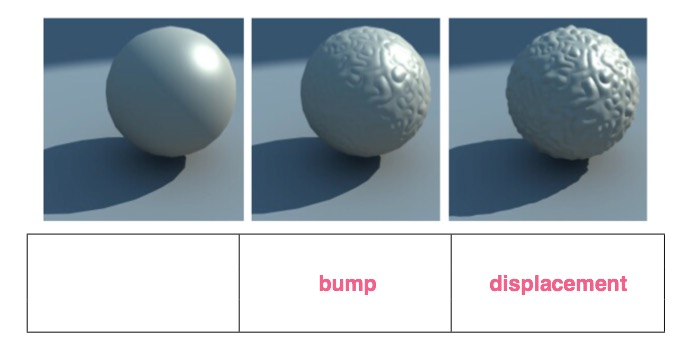
\includegraphics[width=.5\textwidth]{3-2-bump}
\end{figure}
\textit{\textbf{(1points) }Is the bump mapped or the displacement mapped sphere more expensive to render? Why?}\\

Displacement mapping is more expensive since it requires an adaptive tesselation
of the surface to get enough micro-polygons to match the size of a screen pixel.\\

\url{https://en.wikipedia.org/wiki/Displacement_mapping}\\

\textit{\textbf{(1 points)} Using the following figure, show and explain that with perspective projection, barycentric interpolation in screen-space and worldspace differ.
}\\
\begin{figure}[H]
	\centering
	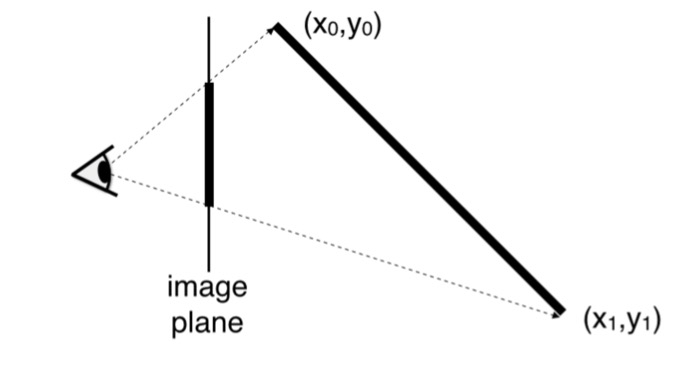
\includegraphics[width=.5\textwidth]{3-2-perspective}
\end{figure}

In screen space: affine math: scaling, tearing and rotating but not perspective (has to be in object space)\\

%TODO explain more clearly

\textit{\textbf{(1 point)} What type of interpolation  does OpenGL employ by default?}\\

%TODO

\textit{\textbf{(1 point)} Which of the two interpolation types is slower to compute for vertex attributes?}\\

%TODO

\textit{\textbf{(3 points)} Why is the correct answer to the previous question not true for interpolating the depth-related information used in the depth test?}\\

%TODO

Because attributes of the form I/z can be linearly interpolated. the depth buffer stores stuff in form const. + 1/z. the const doesn't matter.

\subsection{Mip Mapping}
\textit{\textbf{(2 point)} Which problem does mip mapping address? Why does this problem occur?}\\

Aliasing due to insufficient sampling frequency of the texture. A more remote texture
that has features below the scale of a pixel can show strange artifacts due to the fact that they are „sampled“ incorrectly (avaraged over a pixel). \\

They can also be used to improve the Level of Detail (LoD) of closer objects and speed up rendering
by not rendering remote objects in full resolution\\

\textit{\textbf{(2 points)} How do you compute the mip map texture $T_{n+1}$ from the finer level $T_n$?}\\

construct the texture at a $T_{n+1}$, you filter the $T_n$ with a smoothing kernel and then down- sample it to one forth of the total area.

\textit{\textbf{(3 points)} Show that the increase of storage space required of all mip-map levels is at most one-third of the original texture.}

Every level uses a fourth of the pixels. E.g.,:
$l(1)=64^2,l(2)=32^2...$, therefore the storage requirement of each level is a fourth of its preceding one storage requirement for mipmapping: 

\[\sum_{i=1}^{k\rightarrow\infty}\frac{1}{4^i}=\frac{1}{4^1}+\frac{1}{4^2}+...+\frac{1}{4^\infty}
\]
\[
\begin{aligned}
s&=1/4+1/16+1/64...\\
4*s&=1+1/4...\\
4s&=1+s\\
3s&=1\\
s&=1/3\\
\end{aligned}
\]
Or simply from the geometric series: a=1/4, r=1/4,
then 
\[
\begin{aligned}
a&=1/4, r=1/4\\
s&=\frac{a}{1-r}\\
s&=\frac{1/4}{1-1/4}=\frac{1/4}{3/4}=\frac{1}{3}
\end{aligned}\]

\begin{itemize}
	\item \url{https://en.wikipedia.org/wiki/Geometric_series}
	\item \url{
		https://www.reddit.com/r/math/comments/931jp/a_visualization_of_why_14_116_164_1256_13/}
\end{itemize}
\section{Coding, Lighting, Shading and Rendering Pipeline}
\subsection{Rendering Pipeline}
\textit{\textbf{(7 points)} Mark all the correct statements for OpenGL 3.1. 1 point for marking true statement, -1 point for marking false statement.}
\begin{todolist}
	\item[\done] Depth comparison for shadow mapping is done in fragment shader.
	\item Texture mapping of a triangle is done in geometry shader. Texture mapping of a triangle is done in fragment shader.\\
	\textit{Texture mapping of a triangle is done in fragment shader.}
	\item \texttt{gl\_VertexID} is a built-in output variable of vertex shader.\\
	\textit{\texttt{gl\_VertexID} is a built-in input variable of vertex shader.}	
	\item \texttt{gl\_CameraMatrix} is a built-in input variable of vertex shader. There is no built-in variable gl CameraMatrix.\\
	\textit{There is no built-in variable \texttt{gl\_CameraMatrix.}}
	\item[\done] \texttt{glGenBuffers} is called to find an unused handle for a vertex buffer object.
	\item \texttt{glBufferData} allocates sufficient memory on the CPU for the data. \\
	\textit{\texttt{glBufferData} allocates sufficient memory on the GPU for the data.}
	\item[\done] Rasterizer is NOT programmable by application program.
	\item \texttt{gl\_PrimitiveID} is a built-in input variable of vertex shader. \\
	\textit{\texttt{gl\_PrimitiveID} is a built-in 	input variable of tessellation, geometry and fragment shader.}
	\item[\done] Geometry shader is called after tessellation shader within the same rendering pass. 
	\item[\done] Different stages of the rendering pipeline can run on GPU simultaneously.
	\item[\done] Clipping is done on a primitive-by-primitive basis rather than on a vertex by-vertex basis.
	\item[\done] In OpenGL clipping is done before perspective division.
	\item In OpenGL clipping is done after perspective division.
\end{todolist}

\subsection{OpenGL syntax}
correct order: 
7, 2, 8, 5, 6, 4, 1, 3\\
see \texttt{ex. 2, triangle.h}
\subsection{Phong Lighting}
\textit{The Phong Lighting Model is defined as:}
\[I=I_ak_a+I_dk_d(N\cdot L)+I_sk_s(R\cdot V)^n\]
\textit{where  $N$  is  the  surface  normal,  $L$  the  direction  towards  the  light,  $R$  the  reflection  of  $L$  about  $N$,  and  $V$  is  the  direction  towards  the  camera. $P$ in the sketch is the 3D position of the pixel to be shaded.}\\

\textit{\textbf{(2 points)} Explain the meaning of the following constants:}
\begin{itemize}
	\item $k_a$: ambient color of the material
	\item $I_d$: diffuse intensity of the light
	\item $I_s$: specular intensity of the light
	\item $n$: shininess of the material
\end{itemize}
 \textit{\textbf{(2 points)} Modify the Phong Lighting Model to consider shadows.  Assume you 
have a boolean function \texttt{isInShadow(P)}.}
\[I = I_ak_a + isInShadow(P)(I_d k_d (N \cdot L) + I_sk_s(R \cdot V )n)\]

\subsection{Phong Shading}
\textit{\textbf{(2 points)} Explain the difference between Gouraud and Phong shading. Which one is computationally more expensive. Why?}\\

Shading per vertex vs per pixel.  Phong is more expensive.  Cost:  shade per vertex + interp. a color per pixel vs.  interp. normal (and maybe light dir.) per pixel, renormalize normals,  shade per pixel.
\subsection{Phong Lighting Shader}
\textit{\textbf{(6 points)} Implement the fragment shader of a GLSL program that uses the Phong Lighting Model to render a mesh. You are \underline{not} allowed to define any new uniform or in variables. \textbf{Hint}: Remember to consider back-facing geometry.}\\

\begin{lstlisting}[language=C]
in vec3 normal; // normal in camera space
in vec3 pos; // vertex position in camera space
out vec3 color; // write the final color to this output variable
uniform vec3 light_pos; // light position in eye coordinates
uniform vec3 Ia, Id, Is, ka, kd, ks; 
uniform float n;
void main() {
	color = vec3(0.0) ;
	vec3 ambient = Ia * ka;
	vec3 n = normalize(normal);
	vec3 l = normalize(light_pos);
	float lambert = dot(n,l);
	vec3 diffuse = vec3(0.0, 0.0, 0.0);
	vec3 specular = vec3(0.0, 0.0, 0.0);
	if(lambert > 0.0) {
		diffuse = Id*kd*lambert;
		vec3 v = normalize(pos);
		vec3 r = reflect(-l,n);
		specular = Is*ks*pow(max(dot(r,v), 0.0), alpha);
	}
	color += ambient + diffuse + specular;
}
\end{lstlisting}

\subsection{Shadow Maps}
\textit{\textbf{(1 point)} What kind of projection do you use to generate the shadow map for a point light source? }\\

Perspective projection\\

\textit{\textbf{(2 points)} How should you set the extents of the frustum when you render from the light's point of view to generate the shadow map to achieve best possible quality (least amount of jagged shadow outlines such as the ones shown in the image)?}\\

Tightly around the view frustum and so that points outside the view frustum that can cast shadows into the view frustum\\

\textit{\textbf{(3 points)} For large outdoor scenes, explain what you can do to avoid shadow mapping artifacts similar to the ones in the image above. Assume that your GPU does not support textures larger than 2048 $\times$ 2048.}\\

Cascade shadow maps: high shadow resolution near the camera, low resolution farther away.
\section{Procedural Modeling and Fractals}
\subsection{Measuring the dimensions of fractals}
\textit{\textbf{(2 points)} What is the Hausdorff dimension for fractals, how is it defined?}
\[\begin{aligned}
N&=r^D\\
D&=\log(N)/\log(r)\\
D&=\text{fractal dimension}\\
r&=\text{fractal increment}\\
N&=\text{\# self-similar objects at smaller scale}
\end{aligned}\]
\textit{\textbf{(2 points)} What is the Hausdorff dimension of the 3D quadratic Koch surface (type 2)?}\\

\begin{figure}[H]
	\centering
	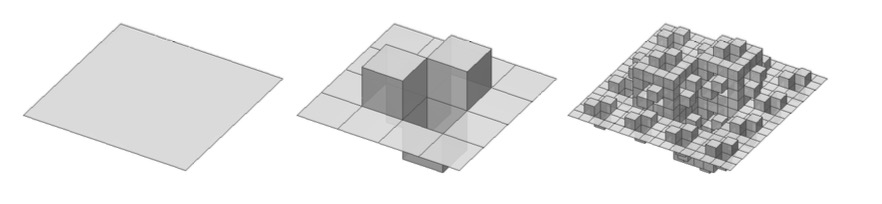
\includegraphics[width=.7\textwidth]{5-koch}
\end{figure}
\[\begin{aligned}
r=4,N=(12+10*2)=32\\
\log(32)/\log(4)=2.5
\end{aligned}\]

\textit{\textbf{(1 point)} What is the Hausdorff dimension of the following fractal: take a unit cube, split it into 27 cubes, keep nine cubes, namely the bottom nine cubes.
}\\

\[\log(9)/\log(3)=2\]

\textit{\textbf{(2 points)} Give formulas for the \underline{volume} and \underline{surface} of the above fractal as a function of the recursion level $k$. What do they converge to for $\lim k\rightarrow\infty$}\\

\textbf{Volume:}
\[\begin{aligned}
v_1&=\Big(\frac{1}{3}\Big)^{1*3}*9^1,v_2=\Big(\frac{1}{3}\Big)^{2*3}*9^2...\\
v_i&=\Big(\frac{1}{3}\Big)^{i*3}*9^i=\Big(\frac{1}{3}\Big)^{i}
\end{aligned}\]
Converges to 0.\\

\textbf{Surface:}
\[
\begin{aligned}
s_1&=\Big(\frac{1}{3}\Big)^{1*2}*6*9^1,s_2=\Big(\frac{1}{3}\Big)^{2*2}*6*9^2...\\
s_i&=\Big(\frac{1}{3}\Big)^{i*2}*6*9^i=\Big(\frac{1}{3}\Big)^{i}=6
\end{aligned}
\]
\subsection{Noise Functions}
\textit{\textbf{(1 points)} When calculating Perlin Noise, the domain is divided into a grid. What are the noise values on the corners of the grid cells?}\\

0 (look at 1d figure)\\

\textit{\textbf{(1 point)} What is the advantage of Perlin Noise over value noise?}\\

Interpolation over tangents and not points, in value noise there is a higher chance that several values in a row
only differ a little. \\

\url{https://computergraphics.stackexchange.com/questions/3608/benefit-of-perlin-noise-over-value-noise/3609}\\

\textit{\textbf{(2 point)} What is Fractal Brownian Motion? Give a short explanation.}

 \begin{itemize}
 	\item Spectral synthesis of noise function
 	\item Progressively smaller frequency
 	\item Progressively smaller amplitude
 	\item Each term in the summation is called an octave
 \end{itemize}
\textit{\textbf{(1 point)} Write down the pseudocode for fBM}
\begin{lstlisting}[language=C]
float fbm (in vec2 st) {
	// Initial values
	float value = 0.0;
	float amplitude = .5;
	float frequency = 0.;
	//
	// Loop of octaves
	for (int i = 0; i < OCTAVES; i++) {
		value += amplitude * noise(st);
		st *= 2.;
		amplitude *= .5;
	}
	return value;
}
\end{lstlisting}

\end{document}